\chapter{多重集合に対するハッシュ値更新アルゴリズム}
本論文では,Datarらのアルゴリズムを動的に変化する多重集合に対して拡張したハッシュ値更新アルゴリズム
SWMH (Sliding-Window Min-Hash)を提案する.
Datarら[1]のアルゴリズムを多重集合に拡張する場合,スライディングウインドウ内の要素$e$への割り当て値が$e$と同じラベルを持つウインドウ内の要素数によって変化する点が難しくなる.つまり,$e$への割り当て値が時間経過によって変化することが起きる.
スライディングウインドウ内の要素$e$のラベルをアルファベット$l(e)$とする.割り当て値$\pi(e)$はスライディングウインドウ内に$l(e)$が何個あるかによって変わる.例えば,図\ref{fig:43}の場合だと,時刻$t=0$の時は,スライディングウインドウ内にアルファベット$b$は2つあり,$\pi(e_i)=4$, $\pi(e_j)$=1となる.時刻$t=3$でスライディングウインドウから要素$e_i$が抜けた場合,$e_j$への割り当て値$\pi(e_j)$は1から4に変化する.
\begin{figure}[H]
  \centering
  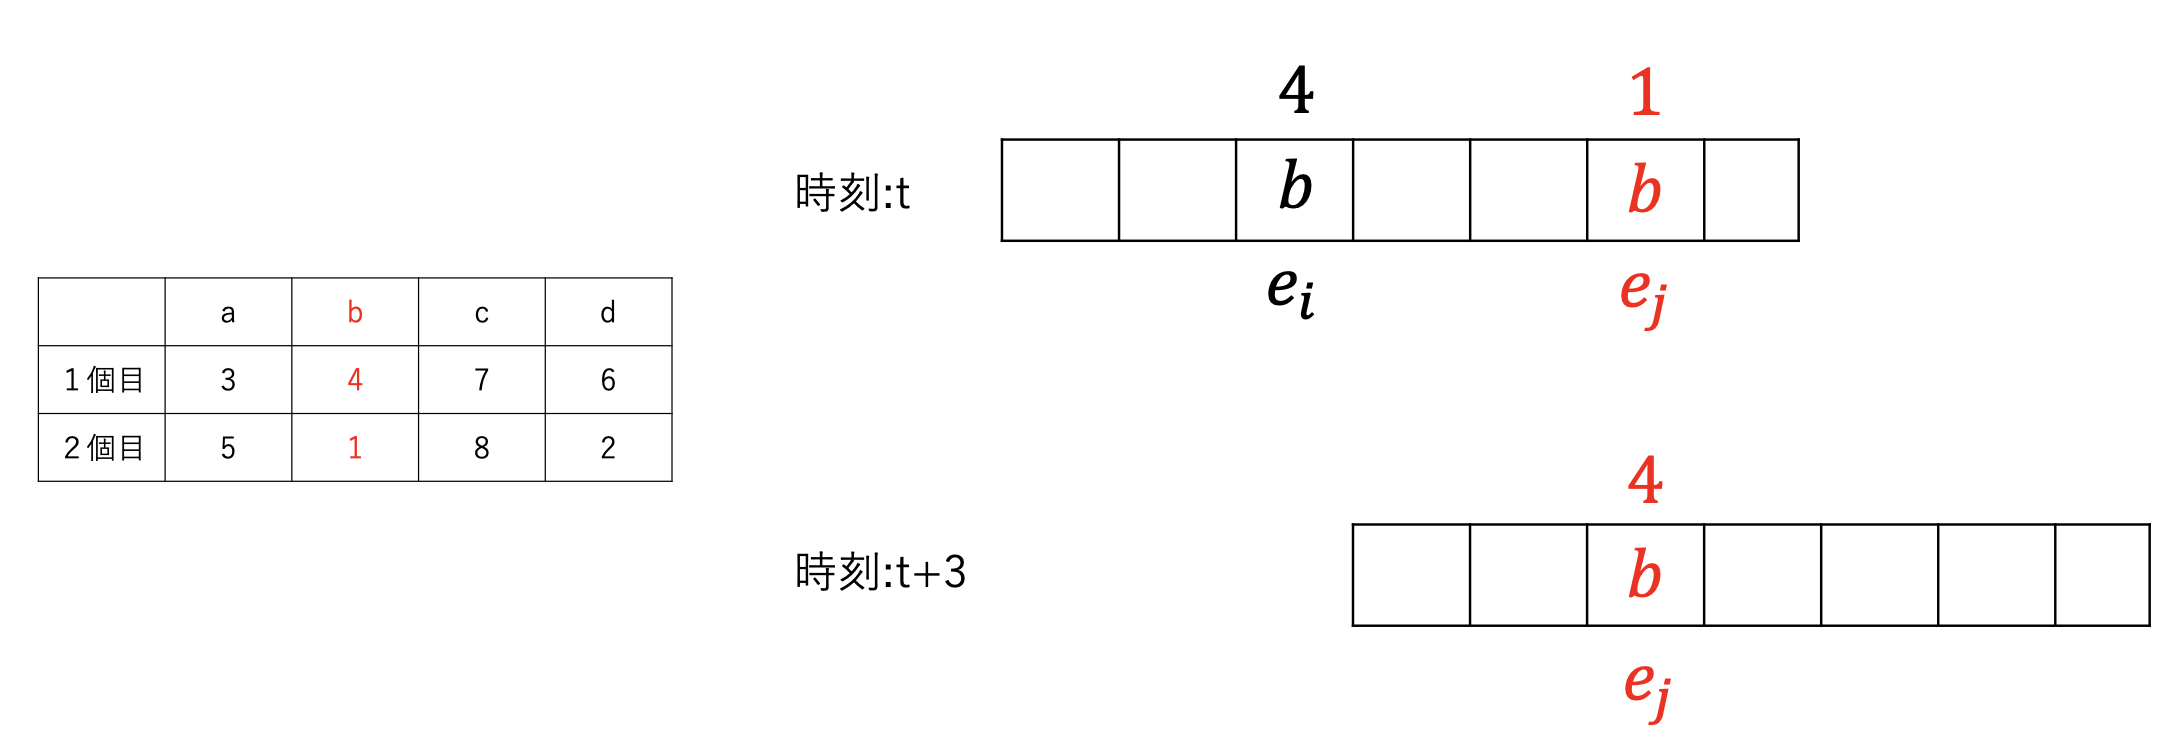
\includegraphics[width=18cm]{43.png}
    \caption{π(e)の変化}
    \label{fig:43}
\end{figure}
Datarらのアルゴリズムでは最小値になり得ない要素をMinlistから削除する.多重集合の場合,割り当て値が
変化することを考慮して最小値になり得るかどうかを判定をする必要がある.提案手法を基盤とする要素技術は
以下の2つであり,それぞれを順に説明する.
\begin{enumerate}
\item 同種アルファベットへの値の割り当て
\item スライディングウィンドウ更新時の処理
\end{enumerate}
%データストリームのスライディングウインドウ内の集合$A_t$が時刻経過により$A_{t+1}$に変化した時,
%R単純な手法は$A_t$を考慮しないでハッシュ値$h(A_{t+1})$を完全に再計算することである.しかし,多重集合に
%対してMin-Hashを何度も再計算をすることは多くの時間を必要とする.
%そして,$A_t$,$A_{t+1}$が多重集合ではなく集合であれば,2.1.2項で述べたDatar[1]らによる動的に変化する集合に対してハッシュ値の更新をするアルゴリズムにより,$h(A_t)$を$h(A_{t+1})$に更新することによって効率よくできる.しかし,このアルゴリズムは多重集合には対応していない.そこで,本研究では,集合に対応しているDatarらのアルゴリズムを多重集合に拡張したSWMHアルゴリズムを提案する.
%\subsection{多重集合の難しさ}
%SWMHではスライディングウインドウの中に同一種のアルファベットが複数存在する場合は到着時刻順に順番を決めている.
\section{同種アルファベットへの値の割り当て}
多重集合に対するMin-Hashでは,多重集合内に同種アルファベットが複数存在する場合それらを区別
して値を割り当てる.例えば,ラベルが$a$のアルファベットが$n$個存在する場合,それらを
$\{a_1,a_2,\cdots,a_n\}$のように区別する.$a_i$ ($1\le i \le $)は$i$番目の$a$という意味であり,
各$a_i$ ($1\le i \le n$)に異なる値$\pi(a_i)$を割り当てる.

ここで$\pi(a_i) \le \pi(a_{i+1})$ならば,$a_{i+1}$の割り当て値は最小には絶対ならない.その理由は
$i+1$番目の$a_{i+1}$が存在する条件下では,$i$番目の$a_{i}$も必ず存在するからである.このように
割り当て値$\pi(a_{i+1})$はMin Hashのハッシュ値に影響を与えないので
$$\pi(a_i) \le \pi(a_{i+1})$$
を条件を満足する限りは別の値に変更しても構わない.そこで,$\pi(a_i) \le \pi(a_{i+1})$が成立する場合は
$\pi(a_{i+1})$を$\pi(a_{i})$に修正する.修正前と修正後を区別するため,修正前の割り当て値を
$\pi(a_{i+1})$とし,修正後の割り当て値を$\pi'(a_{i+1})$とする.

%for文を使ったアルゴリズムの記述と説明。単調減少になることも述べる。Lemma1も載せる。

次にスライディングウィンドウ内の$n$個の$a$のインスタンスをそれぞれ何番目の$a$とするかを
考える.つまり,$n$個の$a$のインスタンスのインデックスをどう定めるかという問題である.
通常の多重集合であれば要素間に時間順序がないのでこの問題は重要でない.しかし、スライディング
ウィンドウの場合,要素間に時間順序があるためインデックスの決め方によって挙動が変わる.自然な
方式としては以下の2つが考えられる.
\begin{itemize}
\item 一番古い要素を$a_1$とし,$a$のインデックスを到着時刻の昇順とする
\item 一番新しい要素を$a_1$とし,$a$のインデックスを到着時刻の降順とする
\end{itemize}

提案手法では,「一番古い要素を$a_1$とし,$a$のインデックスを到着時刻の昇順とする」
という方式を採用する.この時,
\begin{enumerate}
\item $a_i$は$a_{i+1}$より先にデータストリームに到着した
\item $\pi(a_i)\ge \pi(a_{i+1})$
\end{enumerate}
が成立するため,$a_i$は$a_{i+1}$の存在によってMinlistから削除される.
このことが任意の$i$に対して成立するのので,以下のlemma\ref{le:lemma1}が保証される.
%このことが任意の$i$に対して成立するので,Minlistの中に同種アルファベットは最新の1要素しか存在しない事を保証できる.
\begin{lemma}
  \label{le:lemma1}
  Minlistの中に同種アルファベットは最新の1要素しか存在しない.
  \end{lemma}


\begin{lemma}
  \label{le:lemma2}
   $$\min\{\pi(a_1),\pi(a_2),\cdots,\pi(a_n)\} = \min\{\pi'(a_1),\pi'(a_2),\cdots,\pi'(a_n)\}$$
  \end{lemma}



また,lemma \ref{le:lemma2}
が成立するため割り当て値の修正によってハッシュ値は不変である.実際には多重度の上限値$n$をパラメータとして$\pi'$を保持する表を事前計算し,スライディングウィンドウに到着した要素の割り当て値は表を参照して決定する.割り当て表の修正例を図 \ref{fig:44}に示す.この例では多重度の上限が$n=2$であり,2個目の割り当て値が1個目より大きい場合,割り当て値を1個目と同じ値に書き換えている.また,ラベルが$c$の要素$e_i,e_j$の割り当て値の最小値は修正後も修正前から不変になっている.
動的多重集合の場合は,
書き換えによって,Minlistの同じアルファベットの前側の値を消せて,MInlistのサイズを小さくすることができる.




\begin{figure}[H]
  \centering
  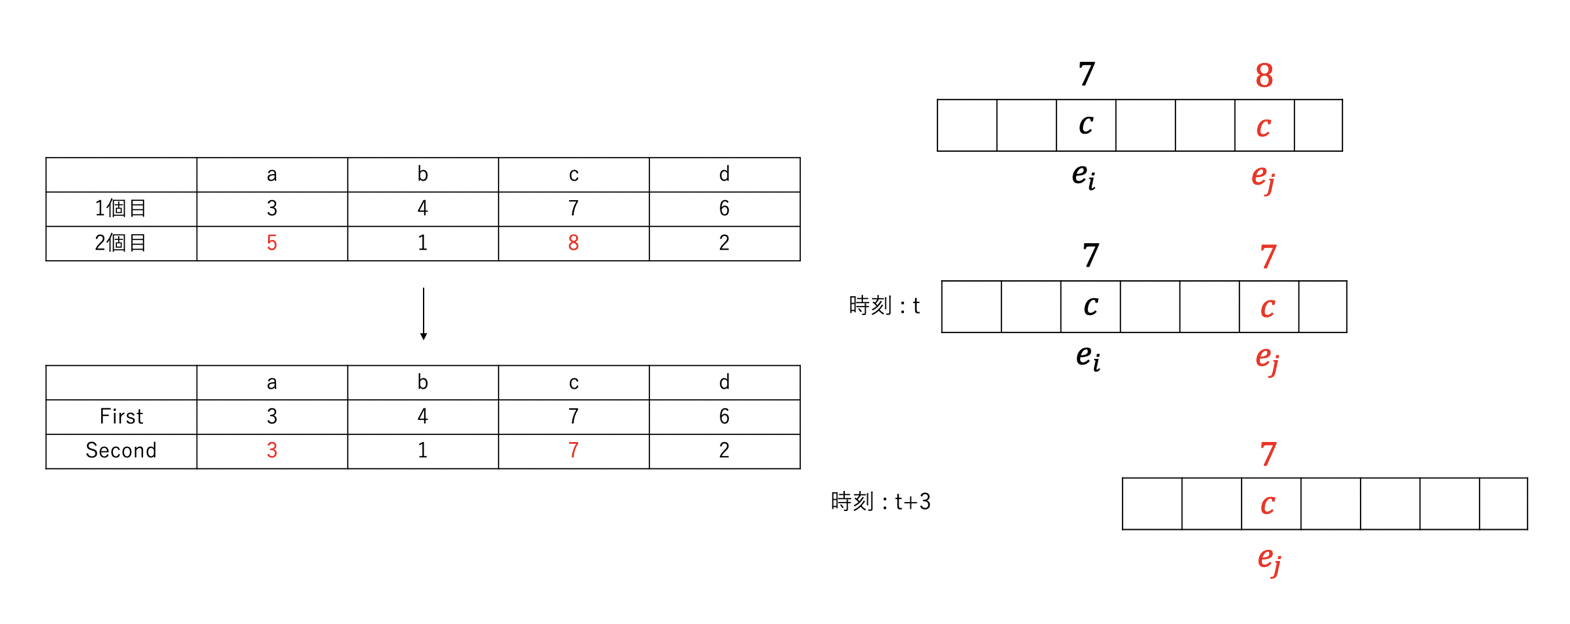
\includegraphics[width=18cm]{44.png}
    \caption{割り当て値の修正}
    \label{fig:44}
\end{figure}
%アルファベットの多重度の上限値が一般に$n(\geq2)$の場合,割り当て表は以下のように1つずつ各アルファベットに対して更新する.
%アルファベットαとする.π($α_1$)よりπ($α_2$)の方が少ない場合もあるが,逆にπ($α_1$)がπ($α_2$)より大きい場合もある.π($α_2$)が小さい場合は,どちらのも値も現在もしくは将来的にハッシュ値になる可能性があるので必要であるが,π($α_2$)が大きい場合,将来的に必要となることがないため,図4.2のようにπ($α_2$)をπ($α_1$)と同じ値で保持する.これは$i$番目でも同じように考えることができ,表にπ($α_i$)を登録する時,π($α_{i-1}$)より大きいか小さいかで上の説明と同じように登録する.
以降では記述を単純化のため,修正後の値割り当て$\pi'$を単に$\pi$と記載する.
\section{ヒストグラムの作成}
%多重集合のスライディングウインドウにおいてMin-hashを更新する場合,
スライディングウインドウが多重集合である場合,スライディングウインドウ内にいくつ同一要素が含まれているかわからないとMin-hashのハッシュ値を計算できない.そこで要素のヒストグラムを保持する.さらに各要素の到着時刻も保持するためヒストグラムのビンを到着時刻のリストとして管理し,リストのサイズにより各アルファベットのスライディングウインドウ内の個数を取得する(図 \ref{fig:4_3_2}).リストは到着時刻が昇順で保持され,新たにウィンドウに到着した要素の到着時刻がエンキューされ,ウインドウから出ていく要素の到着時刻がデキューされる.
%そして,最小値候補リストであるMinlist更新のために,要素がスライディングウインドウに入ってきた時刻とスライディングウインドウ内の要素の個数の2つの情報が必要となる,この2つの情報を保持するために,ヒストグラムは要素の入ってきた時刻をヒストグラムに追加していくように作成した.この作成によって,ヒストグラムの中身で時刻を判断し,ヒストグラムの個数で要素の個数を判断することができる.(図 \ref{fig:4_3_2})
\begin{figure}[H]
  \centering
  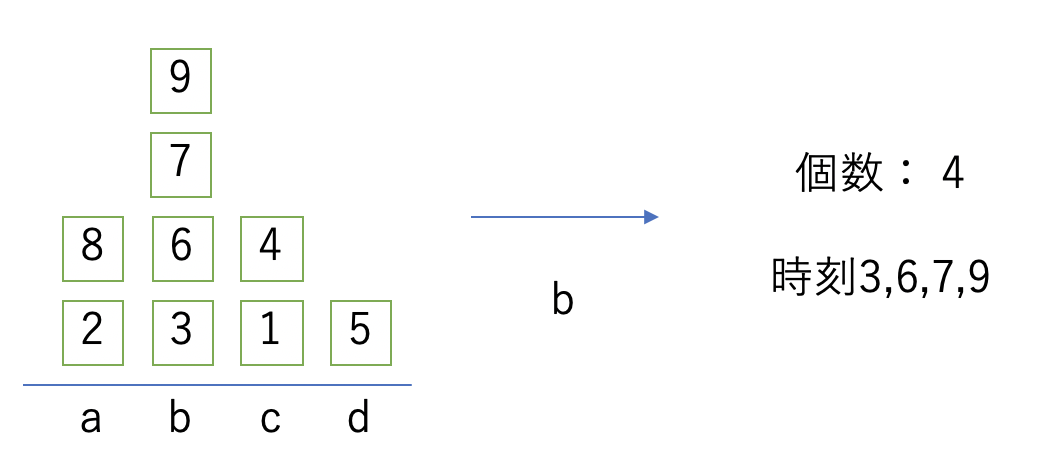
\includegraphics[width=15cm]{4_3_2.png}
    \caption{ヒストグラム}
    \label{fig:4_3_2}
\end{figure}
\subsection{スライディングウインドウの更新}
提案手法SWMHでもDatarらの手法と同様に最小値になりうる要素のリストMinlistを管理する.DatarらのアルゴリズムではMinlistに割り当て値のみを保持していた.
しかし多重集合の場合,割り当て値が変化が発生すると現在の割り当て値から変化後の値を計算できない.変化後の値を計算するため,Minlistは
\begin{itemize}
\item 現在の割り当て値 : $\pi(e)$
\item 要素のラベル : $l (e)$
\item 要素の到着時刻 : $t(e)$
\end{itemize}
の3つ組を要素とするリストとする.
さらにSWMHでは多重集合$A_t$が$A_{t+1}$に変化する時,(1)ウィンドウから一番古い要素$e_{t-w+1}$が離脱する時の
処理と(2)ウインドウに新要素$e_t$に入ってくる時の処理を拡張しなくてはいけない.
%Minlistに.
%しかし,集合の時のように単調増加のリストにはならないため,更新の際に,手間は多くなる.そして,多重集合で行う場合,
\subsection{要素$e_{t-w+1}$がウィンドウから出ていく処理}
%Minlist内で最小割り当て値となる要素$\alpha$のアルファベットを$x$と記述する.
時刻$t$に割り当て値が最小値でハッシュ値と対応する要素を$\alpha$とし,そのラベルを$l(\alpha)$とする.
\noindent (Case 1): Minlistの先頭要素の時刻が$t-w+1$ならばMinlistの先頭要素は$e_{t-w+1}$そのものなのでデキューする.この時,$l(e_{t-w+1}) = l(\alpha)$であったとする.$lemmma$\ref{le:lemma1}より,Minlist内に同じラベルを持つ要素は複数存在しないので$e_{t-w+1}$は$\alpha$と一致する.つまり,ハッシュ値と対応する要素が離脱するため,ハッシュ値の更新が必要となる.
$\alpha$がウィンドウから離脱することになる.そこで,新たに最小割り当て値となる要素をMinlistから探索して更新する.Minlistは割り当て値順にソートされていないので,この操作は
Minlistの全要素のスキャンを伴う.

\noindent (Case 2): Minlistの先頭要素の時刻が$t-w+1$でない場合は$e_{t-w+1}$はMinlistのメンバーではないためMinlistからのデキューは不要である.
しかしこの場合もMinlist内で最小割り当て値が変化する場合がある.具体的には離脱要素$e_{t-w+1}$のアルファベット
が$l({\alpha})$である場合,$l(\alpha)$の多重度が1減るため$\alpha$の割り当て値が増加し,$\alpha$の割り当て値が
ウィンドウ内で最小でなくなる可能性がある.この場合もMinlistをスキャンし新たな最小割り当て値を
探索する.
Case(2)で$e_{t-w+1}$のアルファベットが$l(\alpha)$でない場合,最小割り当て値は不変である.しかし,
Minlist内にラベルが$l(e_{t-w+1})$の要素$\beta$が存在した場合,$\pi(\beta)$は同じラベルの要素数が減少しすることに伴い本来増加する.
しかし,最小割り当て値には影響を与えないのでMinlist内では$\beta$の割り当て値を更新しない.
この結果,Minlist内に保持されている$\beta$の割り当て値は(一時的に)不正確になる.
不正確になった割り当て値の修正は,(Case 2)で最小割り当て値をMinlistをスキャンして更新するときに同時に行う.
正しい割り当て値は$\beta$のアルファベット$l(\beta)$の多重度をヒストグラムから得ることで算出できる.
%先頭要素の時刻が$t$ならば
% アルファベット$x$がMinlistを更新する.最小値の要素がウインドウから出ていく時以外にMinlistを更新しないことによって,Minlistに本来と違う割り当て値で保持される.しかし,割り当て表が単調減少であるため,最小値の選択に影響はなく,毎時刻Minlistを確認する必要がなくなる.間違えている値は,最小値のアルファベットと同じアルファベットがウインドウから出ていく時に一緒に修正する.
% インドウから出ていく時,以下のようにMinlistを更新する.
%
%\begin{itemize}
%\item Minlistの先頭の要素$e_{t+a} (0 \leq a \leq w-1)$,現在の時刻$t_n$,スライディングウインドウの長さ$w$とする.時刻$t(e_{t+a})$と$t_n-w$が一致するならば,Minlistから$e_{t+a}$を削除する.
%\item 現在のハッシュ値を持つ要素のアルファベットとxが一致する場合,Minlistの間違っている割り当て値を修正しつつ,最小値を現在のMinlistの最小値に更新する.
%\end{itemize}
 \subsection{要素$e_{t+1}$をウィンドウに入る時の処理}
$e_{t+1}$がスライディングウインドウに入る時に,Datarらの手法ではMinlistの中で$\pi(e_{t+1})$より
割り当て値が大きい要素を消すだけで十分だった.
しかし,多重集合の場合は$\pi(e_{t+1})$が将来増加する可能性があり,単に$\pi(e_{t+1})$より割り当て値が大きい要素を消すと割り当て値が最小となる可能性がある要素も消してしまう.
そこで,$\pi(e_{t+1})$ではなく,$e_{t+1}$の将来の割り当て
値の上限を上回る要素だけ削除する.$e_{t+1}$のアルファベットを$l(e_{t+1})$とする.
また,Minlist内の要素$\gamma$の到着時刻を$t_{\gamma}$として,$t_{\gamma}$よりあとに到着した
アルファベット$l(e_{t+1})$の個数を$n$とする.$n$の値はヒストグラムの$l(e_{t+1})$のビンに記録された到着時刻
のリストを後方から前方にスキャンすることで求められる.この時,
$$\pi(l(e_{t+1})_{n})<\pi(\gamma))$$
であれば,要素$\gamma$をMinlistから削除してよい.
最後にMinlistの一番後ろに$e_{t+1}$を挿入し,$\pi(e_{t+1})$がMinlistの最小値を更新するかをチェックする.
アルゴリズムの動きをAlgorithm 1に示す.
\begin{figure}[H]
  \centering
  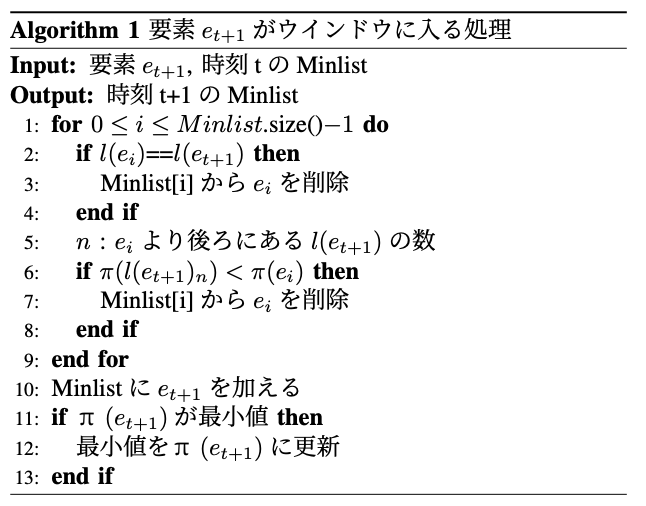
\includegraphics[width=12cm]{4_2_3.png}
    \label{fig:423}
\end{figure}
%e_{w+1}$と同じアルファベットである$\alpha$のスライディ
%ングウインドウ内の個数$n$,割り当て値$\pi$として,$e_{\beta}$よりあとに
%到着した$\alpha$の個数に応じた$\pi$により,将来的に最小値になり得るかど
%うか判断する.以下の処理でMinlistを更新する.

%\begin{figure}[H]
 % \centering
  %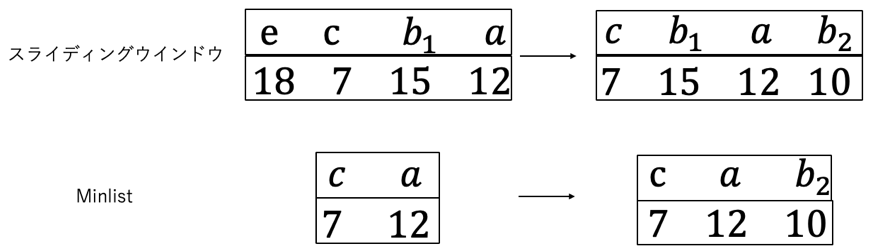
\includegraphics[width=9cm]{45.png}
   % \caption{Minlistの更新}
%\label{fig:minlistupdate}
%\end{figure}
%図\ref{fig:minlistupdate}にMinlistの更新例を示す.

